
\begin{figure*}[t]
  \centering
    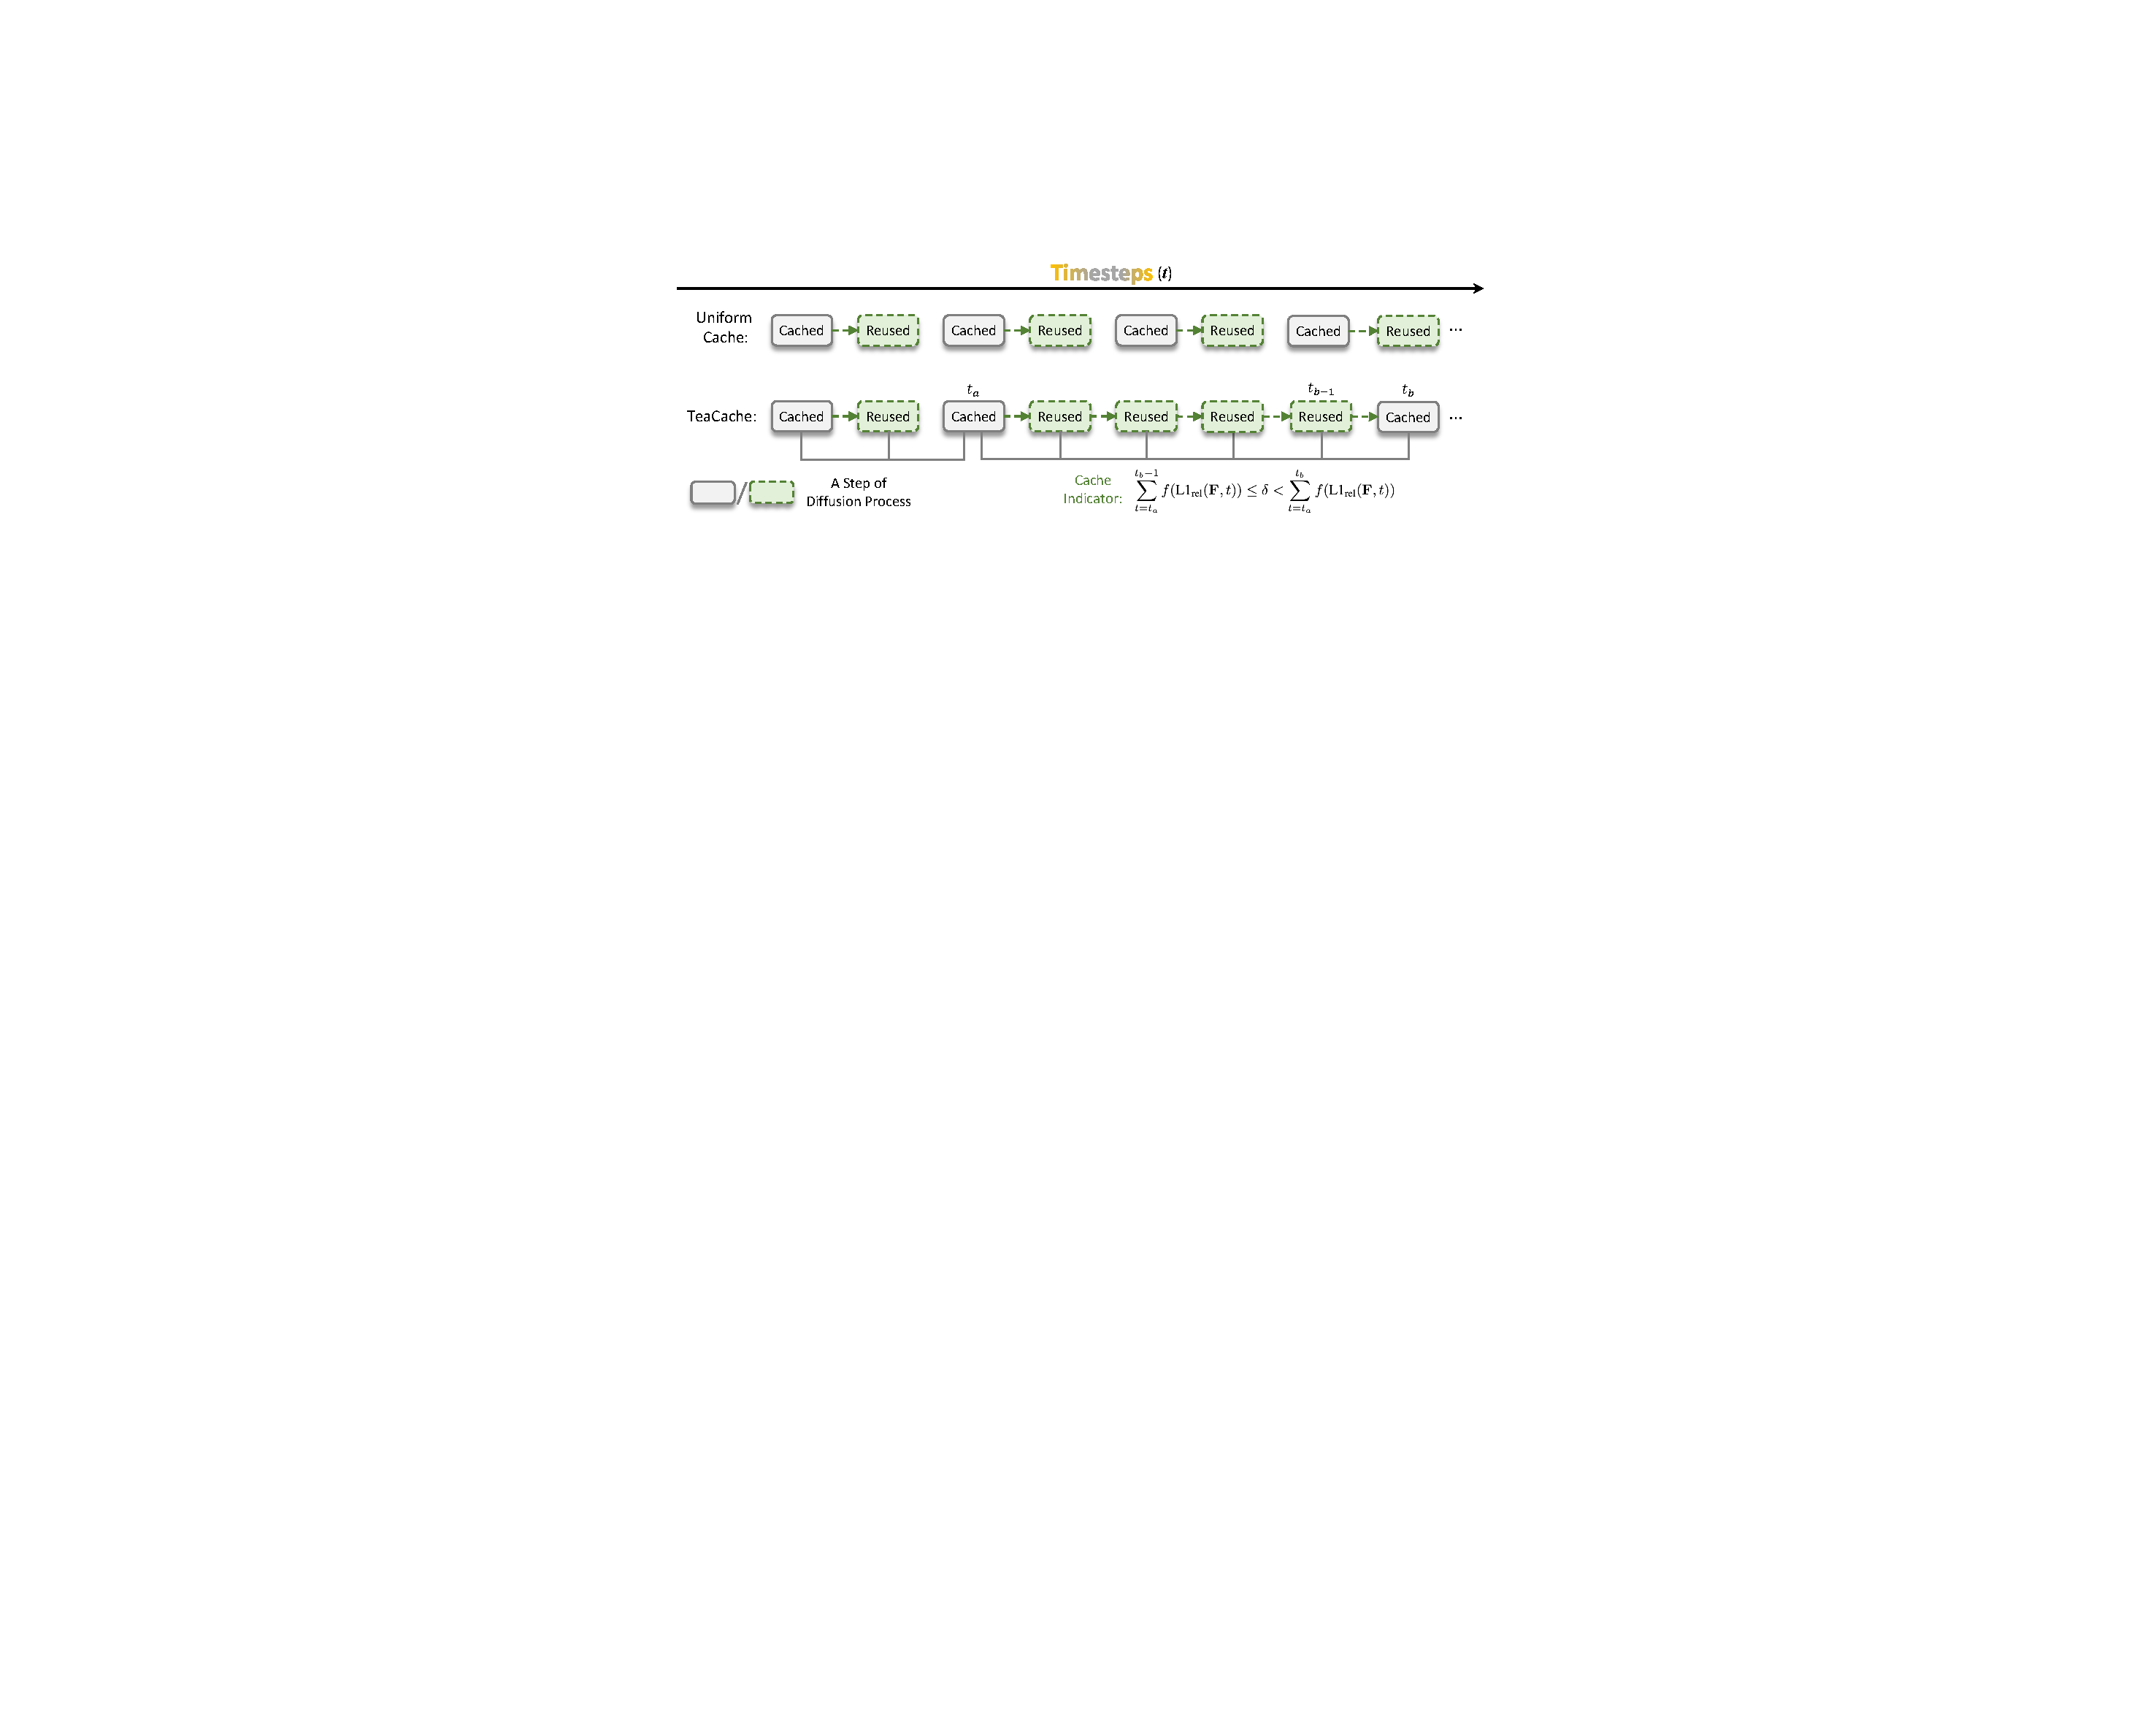
\includegraphics[width=1.0\linewidth]{figs/teacache_arc.pdf}
  \caption{Comparison of the proposed TeaCache and the conventional uniform caching strategy for DiT models during inference. TeaCache is capable of selectively caching informative intermediate model outputs during the inference process, and therefore accelerates the DiT models while maintaining its performance. $\textbf{F}$ and $t$ respectively denote the model inputs of noisy input and timestep embedding. $L1_{rel}$ and $f$ are difference estimation functions of model inputs. $\delta$ is an indicator threshold of whether to cache a model output or not.}
  \label{fig:method_difference}
\end{figure*}

\vspace{-0.5cm}
\section{Introduction}
\label{sec:intro}


% background
Recent years have witnessed the emergence of diffusion models~\cite{dhariwal2021diffusion, ho2020denoising, sohl2015deep, song2019generative}, as a fundamental backbone for visual generation.
The model architecture has evolved from U-Net ~\cite{ramesh2022hierarchical, saharia2022photorealistic, blattmann2023stable} to diffusion transformers (DiT)~\cite{peebles2023scalable}, which greatly increased model capacities.
Empowered by DiT, video generation models~\cite{Open-Sora, Open-Sora-Plan, ma2024latte, yang2024cogvideox, Vchitect, Mochi} 
have reached a groundbreaking level.
% drawback
Despite of the substantial efficacy of these powerful models, their inference speed remains a pivotal impediment to wider adoption~\cite{li2024snapfusion}. This core limitation arises from the sequential denoising procedure inherent to their reverse phase, which inhibits parallel decoding~\cite{shih2024parallel}. Moreover, as model parameters scale up and the requirements for higher resolution and longer durations of videos escalate~\cite{chen2024pixart, yang2024cogvideox}, the inference process experiences a further decline in speed.


% previous solutions
To accelerate the visual generation procedure,
% Fig.~\ref{fig:shot}, 
distillation~\cite{sauer2023adversarial, wang2023videolcm, meng2023distillation} and post-training~\cite{chen2024q, ma2024learning} are employed. 
However, these methods typically require extra training, which implies substantial computational cost and data resources.
%
An alternative technological pathway is to leverage the caching mechanism~\cite{smith1982cache, goodman1983using, albonesi1999selective}, which does not require additional training to maintain the performance of diffusion models.
%
These methods~\cite{xu2018deepcache, selvaraju2024fora, zhao2024real, chen2024delta} find that the model outputs are similar between the consecutive timesteps when denoising and propose to reduce redundancy by caching model outputs in a uniform way, Fig.~\ref{fig:method_difference}(upper).
%
Nevertheless, when the output difference between consecutive timesteps varies, the uniform caching strategy lacks flexibility to maximize the cache utilization.

% our goal, different
In this study, we aim to develop an novel caching approach by fully utilizing the fluctuating differences among outputs of the diffusion model across timesteps.
%
The primary challenge is: when can we reuse cached output to substitute the current timestep's output? Intuitively, this is possible when the current output is similar with the cached output, Fig.~\ref{fig:method_difference}(upper).
%still
Unfortunately, such difference is not predictable before the current output is computed. Consequently, without the guidance of difference, the uniformly cached outputs becomes redundant and the inference efficiency remains low.

% our solution, is always
To conquer this challenge, we propose Timestep Embedding Aware Cache (TeaCache), a training-free caching strategy. TeaCache leverages the following prior: {\textbf{\textit{There exists a strong correlation between a model's inputs and outputs.}} If a transformation relationship can be established between the input and output difference, one can utilizes the difference among inputs as an indicator of whether the corresponding outputs need to be cached, Fig.~\ref{fig:method_difference}(lower). 
%
Since inputs are readily accessible, this approach would significantly reduce computation cost.
%
We then delve into the inputs of diffusion models: a noisy input, a timestep embedding, and a text embedding. The text embedding remains constant throughout the denoising process and cannot be used to measure the difference of input across timesteps.
%
As for the timestep embedding, it changes as timesteps progress but is independent of the noisy input and text embedding, making it difficult to fully reflect the input information. 
%
The noisy input, on the other hand, is gradually updated during the denoising process and contains information from the text embedding, but it is not sensitive to timesteps. 
%
To accurately describe the model inputs and ensure their strong correlation with the outputs, TeaCache follows the inference process of diffusion and employ the timestep-embedding modulated noisy input
as the final input embeddings, among which the difference are then used to estimated the output difference. 


It is noteworthy that the input difference estimated above still exhibits a scaling bias relative to the output difference, which has been observed through empirical studies. That is because this strategy only captures the correlation trend between input difference and output difference. Considering that both input and output differences are already scalars, TeaCache further introduces a simple polynomial fitting procedure to estimate the scaling factors between them. 
%
With the correction of the scaling factors, the input difference can accurately reflect the output difference and is ultimately used as an indicator of whether the outputs need to be cached, Fig.~\ref{fig:method_difference}(lower).
%low给人的感觉是相似性低,是不是可以直接说他们是scalar


% summary
The contributions of this paper include:
\begin{itemize}[leftmargin=*]
    \item We propose TeaCache, a training-free approach which is completely compatible with DiT diffusion models, to estimate the difference of model outputs, selectively cache model outputs and speed up the inference process. 
    \item We propose a simple-yet-effective two-stage strategy to estimate the difference of model output through model input. The proposed strategy uses timestep-embedding modulated noisy input to perform coarse estimation and a polynomial fitting procedure for refinement.
    \item TeaCache speeds up SOTA generation models, Open-Sora \cite{Open-Sora}, Open-Sora-Plan \cite{Open-Sora-Plan}, and Latte \cite{ma2024latte}, (PAB~\cite{zhao2024real}) with large margins at negligible quality cost, Fig.~\ref{fig:shot}.
\end{itemize}

